% !TEX TS-program = pdflatex
% !TEX encoding = UTF-8 Unicode

% This is a simple template for a LaTeX document using the "article" class.
% See "book", "report", "letter" for other types of document.

\documentclass[11pt]{article} % use larger type; default would be 10pt

\usepackage[utf8]{inputenc} % set input encoding (not needed with XeLaTeX)

%%% Examples of Article customizations
% These packages are optional, depending whether you want the features they provide.
% See the LaTeX Companion or other references for full information.

%%% PAGE DIMENSIONS
\usepackage{geometry} % to change the page dimensions
\geometry{a4paper} % or letterpaper (US) or a5paper or....
% \geometry{margin=2in} % for example, change the margins to 2 inches all round
% \geometry{landscape} % set up the page for landscape
%   read geometry.pdf for detailed page layout information

\usepackage{graphicx} % support the \includegraphics command and options

% \usepackage[parfill]{parskip} % Activate to begin paragraphs with an empty line rather than an indent

%%% PACKAGES
\usepackage{booktabs} % for much better looking tables
\usepackage{array} % for better arrays (eg matrices) in maths
\usepackage{paralist} % very flexible & customisable lists (eg. enumerate/itemize, etc.)
\usepackage{verbatim} % adds environment for commenting out blocks of text & for better verbatim
\usepackage{subfig} % make it possible to include more than one captioned figure/table in a single float

% These packages are all incorporated in the memoir class to one degree or another...

%%% HEADERS & FOOTERS
\usepackage{fancyhdr} % This should be set AFTER setting up the page geometry
\pagestyle{fancy} % options: empty , plain , fancy
\renewcommand{\headrulewidth}{0pt} % customise the layout...
\lhead{}\chead{}\rhead{}
\lfoot{}\cfoot{\thepage}\rfoot{}

%%% SECTION TITLE APPEARANCE
\usepackage{sectsty}
\allsectionsfont{\sffamily\mdseries\upshape} % (See the fntguide.pdf for font help)
% (This matches ConTeXt defaults)

%%% ToC (table of contents) APPEARANCE
\usepackage[nottoc,notlof,notlot]{tocbibind} % Put the bibliography in the ToC
\usepackage[titles,subfigure]{tocloft} % Alter the style of the Table of Contents
\renewcommand{\cftsecfont}{\rmfamily\mdseries\upshape}
\renewcommand{\cftsecpagefont}{\rmfamily\mdseries\upshape} % No bold!

%%% END Article customizations
 \usepackage{fixltx2e}





%%% The "real" document content comes below...

\title{Visual Rendering \& Oculus Rift}
\author{Marco Godi \& Francesco Giuliari}
%\date{} % Activate to display a given date or no date (if empty),
         % otherwise the current date is printed 

\begin{document}
\maketitle


\tableofcontents





%%%%%%%%%%%%%%%%%%%%%%%%%%%%%
%%%%%        Introduction        %%%%%%%%%%%%%%
\newpage
\section {Introduction}
The scope of this project is to make a Volumetric viewer compatible with the Oculus Rift headmount display.

%%%
\subsection{Volumetric rendering}
Volumetric rendering is the name used to describe techniques used to display a 2D projection of a 3D data set. It differs from ``normal'' rendering Techniques because while more costly it offers more the opportunity to interact with the 3D model so we can split the model, see his internal components and overall get more information at run time.  

%%%
\subsection{The Oculus Rift}
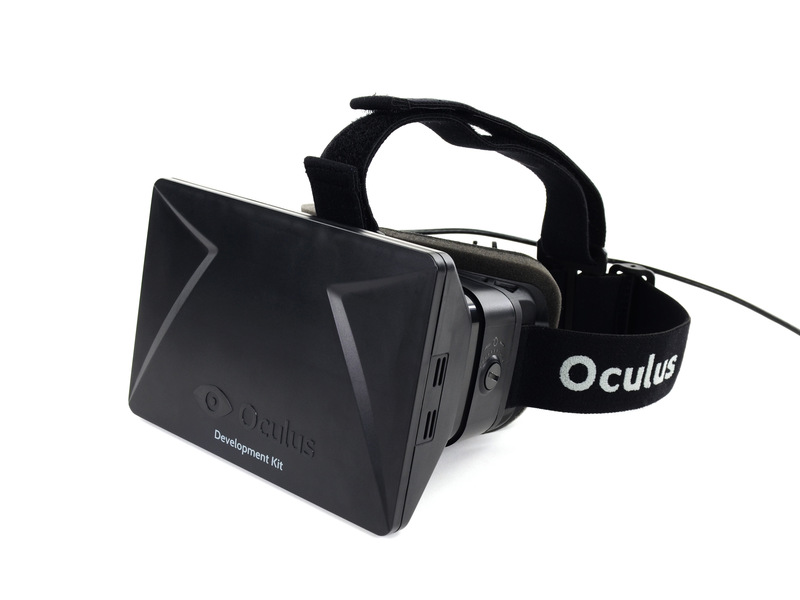
\includegraphics[scale=0.5]{oculus.jpg}

The Oculus Rift  is a virtual reality headset by Oculus VR that offer the user a fully immersive experience so they can see and interact with the application as if he was seeing with his own eyes instead of looking at a monitor. As of today the most advanced model is the DK2, for this project we're using the DK1. Our application is not compatible with DK2 because the approach we used is not supported on the newer model and the updated approach needs a more in-depth knowledge of the OpenGL pipeline. Luckily anyone with the required knowledge can make our application compatible by modifying the code where the distortion is applied (More details on later sections).






%%%%%%%%%%%%%%%%%%%%%%%%%%
%%%       Requirements         %%%%%%%%%%%%%



\newpage
\section{Requirements}

%%%
\subsection{Hardware}
\begin{itemize}
\item It needs a fairly powerful computer (expecially a powerful video card) to run smoothly because the Volumetric rendering is a resources hungry technique and, since the oculus needs to have a different texture for both of the eyes, the rendering cost doubled.

\item The graphic card needs to be able to use OpenGL 3.1 .

\item Oculus Rift DK1 or DK2
\end{itemize}


%%%
\subsection{Software}
\begin{itemize}
\item The application at the moments only supports Windows operationg system since it uses OS dependant libraries, it was developed and tested on Windows 8.1.
\item To succesfully use the Oculus Rift headest the needs to have the Oculus Runtime software available at the Oculus VR official site.
\end{itemize}












%%%%%%%%%%%%%%%%%%%%%%%%%%%
%%             External Libraries               %%%%%%%%%%

\newpage
\section{External Libraries}
Since this project needed to be completeted in a fairly reasonable amount of time we decided to use some external libraries for an easier management, for the volumetric rendering we're using the VTK libraries, and, for the Oculus Rift management we're using the Oculus SDK libraries

%%%
\subsection{VTK}
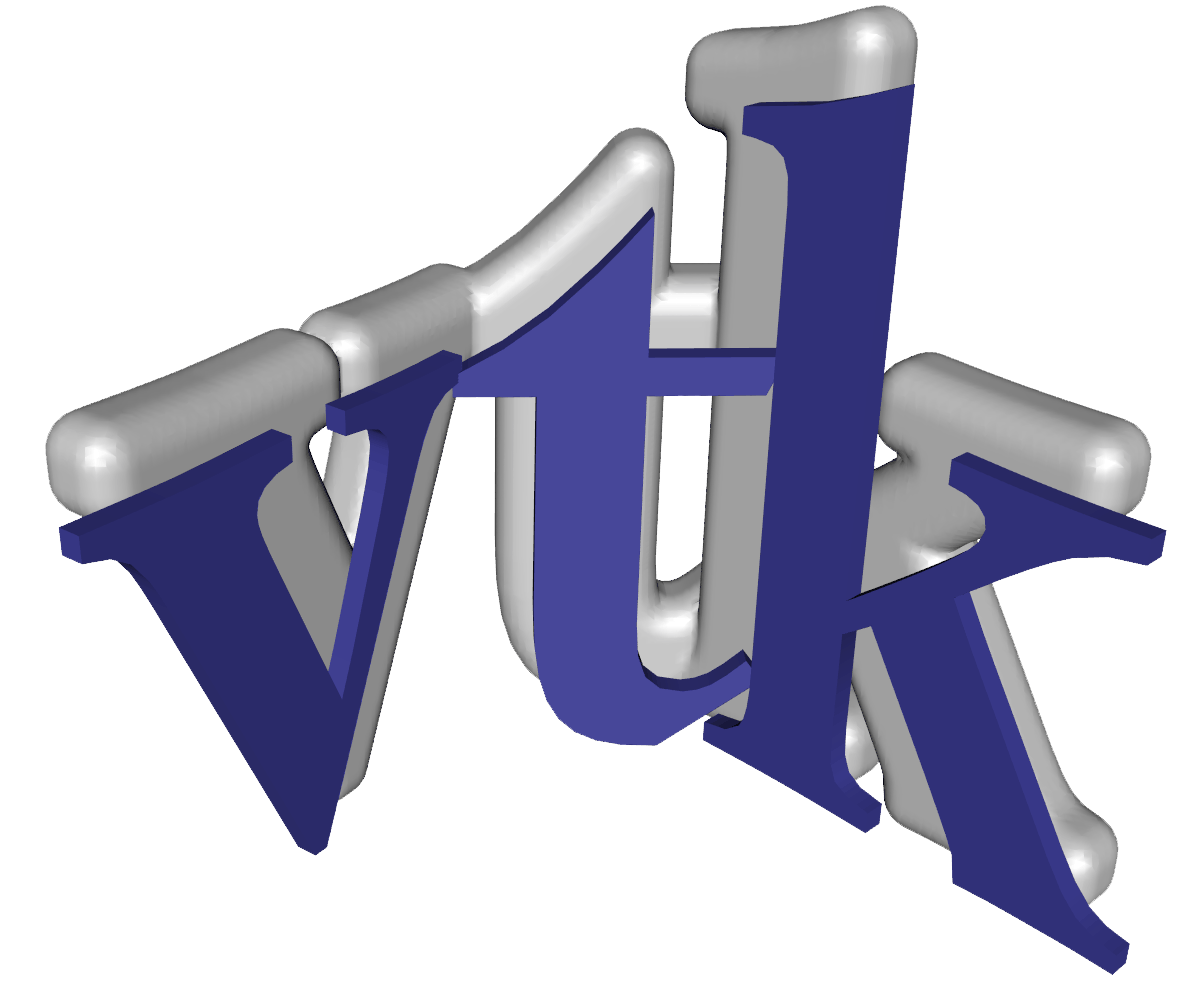
\includegraphics[width=0.2\linewidth]{VTK.png}

The Visualization Toolkit (VTK) is an open-source, freely available software system for 3D computer graphics, modeling, image processing, volume rendering, scientific visualization, and information visualization. VTK also includes ancillary support for 3D interaction widgets, two- and three-dimensional annotation, and parallel computing. At its core, VTK is implemented as a C++ toolkit, requiring users to build applications by combining various objects into an application. The system also supports automated wrapping of the C++ core into Python, Java, and Tcl, so VTK applications may also be written using these interpreted programming languages.

%%%%
\subsection{Oculus SDK}
\includegraphics[width=0.4\linewidth,clip,trim=7cm -3mm 5cm -2mm]{Oculus_sdk.png}

The Oculus SDK is the libraries offered by Oculus VR to manage Oculus Rift headset implementation. It offer methods to keep tracking of the headpose, obtain hardware specifics form the Oculus headset and it allow for creation of virtual heaset useful for debugging the application.










%%%%%%%%%%%%%%%%%%%%%%%%%%%%
%%%%%%%    Project     %%%%%%%%%%%%%%%%



\newpage
\section{Project}

%%%
\subsection{Approach}
The application uses the VTK libraries to load the Dicom files (or MHA or VTI files) which are to be visualized as a 3D dataset by a volumetric algorithm, then creates a split screen which shows two different points of view of the visualized dataset (representing the two eyes of the user) with the appropriate distance determined by the eye spacing and then applies a barrel distortion shader so that the image is fixed to display properly on the Oculus Rift.

%%%
\subsection{Classes}
\begin{description}

\item[Main] \hfill \\
  This class import the DICOM files and create the volumetric viewport.
   \item[Rift\_Pass] \hfill \\
  This class apply the barrel distortion shader.
  \item[Split\_window] \hfill \\
  This class create two viewports from a single one and keep them synchronized.
  \item[Oculus\_middleware] \hfill \\
  This class is used as a class used to initializate the Oculus and return hardware related information such as the head pose and textures size.

\end{description}



%%%%%%%%%%%%%%%%%%%%%%%%%%%%%%
%%%%%%%  Development Journal     %%%%%%%%%%%%
\newpage

\section{Development journal}
Over the course of this stage we had to go through many stages in which we were faced with different problems each one with many alternative solution. In this section will be posted which of these solutions were implemented in the project and the reasons for its choosing. 

%%%
\subsection{Volumetric rendering libraries}
The first thing we had to decide was how to handle the volumetric rendering, the possible libraries are linked below

\begin{description}

\item[Voreen]\hfill \\ 
 Voreen is an open source rapid application development framework for the interactive visualization and analysis of multi-modal volumetric data sets. It provides GPU-based volume rendering and data analysis techniques and offers high flexibility when developing new analysis workflows in collaboration with domain experts. The Voreen framework consists of a multi-platform C++ library, which can be easily integrated into existing applications, and a Qt-based stand-alone application.
 \item[VTK] \hfill \\
The Visualization Toolkit (VTK) is an open-source, freely available software system for 3D computer graphics, modeling, image processing, volume rendering, scientific visualization, and information visualization. VTK also includes ancillary support for 3D interaction widgets, two- and three-dimensional annotation, and parallel computing. At its core, VTK is implemented as a C++ toolkit, requiring users to build applications by combining various objects into an application. 
 \item[Open Inventor] \hfill \\
Open Inventor® is an object-oriented, cross-platform 3D graphics toolkit for the development of industrial-strength, interactive applications using C++, .NET or Java.
Its easy-to-use API, its extensible architecture, and its large set of advanced components provide developers with a high-level platform for rapid prototyping and development of 3D graphics applications.

\end{description}

\noindent
After a long discussion among ourselves where we studied the pros and cons of each library we decided to use the VTK libraries mainly for these two reason :
\begin{itemize}
\item Vooren, while offering a whole framework and many already implemented function, has almost no documentation and we didn't have enough time to learn it from scratch. %questa frase non mi convince, todo cambiarla
\item Open inventor is not open sourced. 
\end{itemize}

%%%
\subsection{Omegalib}
Now that we decided to use the VTK as volumetric rendering library, we looked up projects similar to this one so we could use that as a base or as an inspiration.After a little search we found a project that seems to be the silver bullet for our problem, that being Omegalib by UIC Electronic Visualization Laboratory.
\newline
\newline
The main features that leaded us to try using Omegalib are:
\begin{itemize}
\item It implements two rendering libraries, OpenSceneGraph and VTK.
\item It natively redirects  the output on various devices, among them is the OculusRift.
\item Support for a wide range of input peripherals (controllers, motion  capture systems, touch surfaces, speech and brain interfaces), through  the  Omicron toolkit.
\item It offers a python wrapper so that the program could be written using a simpler language.
\end{itemize}

\noindent
We decided that learning to use the Omegalib was our best bet to make this project easier to extend for future development, so we rewrote our vtk application as a python script.
On paper the last thing that needed to be done was assigning the oculus rift configuration to the application, but when we tried doing that it didn't work and the results weren't as expected.
We attempted  reviewing the whole library code that manage the output control, specifically how it interacted with the oculus rift configuration and then contacted the Omegalib developer on the project mailinglist to see if there was a way to see what the problem was and how to resolve it.
Turns out that, while Omegalib implements the VTK, it doesn't support the volumetric rendering, at least it doesn't as of now, it may be implemented in the future.

Because of this any and all plans of using Omegalib for this project fell through so we were back at the beginning and had to go with pure VTK again.

So what we needed was to find a way to implement all of these features:
\begin{itemize}
\item Volumetric Visualization of 3D datasets
\item "Two points of view" management (for the two eyes of the Oculus user)
\item Applying barrel distortion
\item Inserting head pose tracking into a VTK application
\item Outputting video on the Oculus Rift
\end{itemize}

%link qui o li mettiamo in fondo nelle citazioni? MI DA ERRORE QUA NON SO COSA
%We looked for other similar projects and two caught our attention: multipass_vtk by zadacka ( https://github.com/zadacka/multipass_vtk ) and and application by  Przemysław Brudny and Mateusz Wójcik by the Universidade de Aveiro ( which you can find here http://sweet.ua.pt/paulo.dias/rva/TrabalhosRVA_2.htm ).
The first one sadly only supports Linux and uses an older version of  the Oculus SDK, but uses an interesting approach (the multipass system offered by VTK) which we'll look more into later.
The second one also uses an older version of the Oculus SDK. Also it uses a software distortion of the image, making it too slow for an interactive experience.
While we were studying these projects, we started developing other components of our software.
Starting from a VTK example, we created a Volumetric viewer which takes a series of .dcm files (or a .vti or a .mha) and visualizes it on screen, making it possibile to manipulate it by moving the camera and using widgets to make cross sections of it in real time.
%screen del Volumetric Viewer
While we were looking into a way to apply a barrel distortion and output our software onto the Oculus Rift, we also created a program which visualized onto two viewports on a split screen a normal VTK application, each viewport having a translated camera based on the eye distance value. We made this software and it worked, but then we discarded it because we found another solution, easier to manage and less verbose.
We also looked into pre-existing OpenGL Oculus Rift applications to get an idea about how to make a VR software. We found very soon that the latest way to do it involved pure OpenGL which is very problematic to use in a VTK application without knowing it very well because you could mess withthe VTK pipeline. So we opted for a deprecated way, which includes distortion using a shader in post-processing and using Mirrored Desktop so you can use the Oculus as an external monitor.
So we learned of two ways to apply post processing into a VTK application:
\begin{itemize}
\item The external way: WindowToImageFilter, which "takes a screenshot" of a viewport and lets you use it as an Actor2D... Two problems: it's very slow (it loads the screenshot from video memory to RAM and the to video memory again) and also doesn't support shaders.
%DIO CANE DA ERRORE LA SCRITTA MULTIPASS
\item The internal way: Multipass ( inspired by zadacka's multipass\_vtk ) which lets you build the rendering pipeline of an application, sometimes down to the OpenGL code. Using a Gaussian Blur Post Processing example as a starting point we built a class which solves two of our needed features: "Two points of view" (by making the render pass render the scene two times from different positions) and barrel distortion (by applying a shader to the texture in which we store the rendered scene).
\end{itemize}
So we had a volumetric viewer, we could have video from our two eyes, we could distort it and output all of this into our Oculus Rift by mirroring the screen.
We only needed to handle the user's Head Pose, which we did by polling it trough the Oculus SDK every few milliseconds.




\end{document}
